This chapter provides an overview of the terms and techniques used in this chapter.
This chapter starts with an introduction on \acp{ANN}, their structure and their value in \ac{CPS}.
The aim is to provide a general understanding to the functionality of \acp{ANN} and their safety regarding \ac{CPS}.
The next section briefly introduces synchronous programming, and highlights Esterel as the language of choice for this thesis. 
An example of an Esterel program is given, with a quick run-down of how it functions and its syntax.
The chosen method of \acf{WCET} analysis is discussed.
Finally, \ac{RE} is introduced as a safety mechanism for \ac{CPS}.

The related work concerning the convergence of formal methods and \acp{AI} is introduced.
This covers the verification and validation of \ac{ANN}, and the timing and functional safety of these \acp{ANN}.

\section{Background}
\subsection{\acfp{ANN}}
\acp{ANN} were originally proposed to mimic the functioning of  biological neural networks~\cite{kohonen1988introduction}, which produce recurrent spatio-temporal patterns~\cite{rolston2007precisely}. 
Similar timed activity of neurons in the cerebellum has been reported in~\cite{bullock1994neural, moore1989adaptively}. 
A number of types of \ac{NN} which mimic their biological counterparts exist, varying in complexity and accuracy, including the \ac{SNN}~\cite{izhikevich2003spiking,maass1997spiking}, which was designed to model the brain and has been demonstrated to be periodic and run with discrete time intervals when implemented in software. 
\acp{ANN} are also part of deep learning; \acfp{CNN}~\cite{schmidhuber2015deep} were introduced with many more layers than is possible on a \ac{MLP}. 
\acp{CNN}, are widely used in \ac{CPS} applications such as autonomous vehicles, e.g. in \cite{EndToEndLearningForSelfDrivingCars}, where a \ac{CNN} is trained to map raw pixel data directly to vehicle steering commands.

\subsubsection{Structure of an \acf{ANN}}
Most \acp{ANN} do not feature such complex models like those of spiking neural networks, as they are more difficult to use, implement, and train. 
Instead, they rely on simpler networks, which can be considered as \emph{un-timed non-linear} functions, where the outputs change relative to the inputs, but the timing of the change is not precisely defined. 
An example of such a network is provided in Figure~\ref{fig:mlp-ann}, which is using neurons defined in Figure~\ref{fig:artificial-neuron}. 
This is a type of \ac{ANN} known as an \acf{MLP}~\cite{yegnanarayana1994artificial}.
A \ac{MLP} consists of interconnected layers of artificial neurons, each neuron providing input to neurons in the next layer~\cite{grad-desc}.

\begin{figure}[h]
	\centering
	\scalebox{0.8}{\def\layersep{2.25cm}
\def\numInp{4}
\def\numHid{5}
\def\numOut{3}
\begin{tikzpicture}[shorten >=1pt,->,draw=black!100, node distance=\layersep]
	\tikzstyle{every pin edge}=[<-,shorten <=1pt]
	\tikzstyle{neuron}=[circle,fill=black!25,minimum size=20pt,inner sep=0pt]
	\tikzstyle{input neuron}=[neuron, fill=white!100,draw=black];
	\tikzstyle{output neuron}=[neuron, fill=white!100,draw=black];
	\tikzstyle{hidden neuron}=[neuron, fill=white!100,draw=black];
	\tikzstyle{annot} = [text width=4em, text centered]
	
	% Draw the input layer nodes
	\foreach \name / \y in {1,...,\numInp}
	% This is the same as writing \foreach \name / \y in {1/1,2/2,3/3,4/4}
	\node[input neuron, pin=left:Input \y] (I-\name) at (0,-\y) {$i_\y$};
	
	% Draw the hidden layer nodes
	\foreach \name / \y in {1,...,\numHid}
	\path[yshift=0.5cm]
	node[hidden neuron] (H-\name) at (\layersep,-\y cm) {$h_\y$};
	
	% Draw the output layer nodes
	\foreach \name / \y in {1,...,\numOut}
	\node[output neuron, pin={[pin edge={->}]right:Output \y}] (O-\name) at (4.5,-0.25-\y) {$o_\y$};
		
	% Connect every node in the input layer with every node in the
	% hidden layer.
	\foreach \source in {1,...,\numInp}
	\foreach \dest in {1,...,\numHid}
	\path (I-\source) edge (H-\dest);
	
	% Connect every node in the hidden layer with the output layer
	\foreach \source in {1,...,\numHid}
	\foreach \dest in {1,...,\numOut}
	\path (H-\source) edge (O-\dest);
	
	% Annotate the layers
	\node[annot,above of=H-1, node distance=1cm] (hl) {\textit{Hidden Layer}};
	\node[annot,left of=hl] {\textit{Input Layer}};
	\node[annot,right of=hl] {\textit{Output Layer}};
\end{tikzpicture}}
	\caption{Example \ac{MLP} \ac{ANN}, showing the layers of artificial neuron and their connections.	\label{fig:mlp-ann}}
\end{figure}
\begin{figure}[h]
	\centering
	\scalebox{0.8}{\begin{tikzpicture}[
init/.style={
  draw,
  circle,
  inner sep=2pt,
  font=\Huge\itshape,
  join = by -latex
},
squa/.style={
  draw,
  inner sep=2pt,
  font=\Large,
  join = by -latex
},
start chain=2,node distance=10mm
]
\node[on chain=2] 
  (x2) {$x_2$};
\node[on chain=2,join=by o-latex] 
  {$w_2$};
\node[on chain=2,init] (sigma) 
  {$\displaystyle\Sigma$};
\node[on chain=2,squa,label=above:{\parbox{2cm}{\centering \textit{Activation \\ function}}}]   
  {$f$};
\node[on chain=2,label=above:\textit{Output},join=by -latex] 
  {$y$};
\begin{scope}[start chain=1]
\node[on chain=1] at (0,1cm) 
  (x1) {$x_1$};
\node[on chain=1,join=by o-latex] 
  (w1) {$w_1$};
\end{scope}
\begin{scope}[start chain=3]
\node at (0.9, -1.2cm) (dots) {...};
\node[on chain=3] at (0,-2cm) 
  (x3) {$x_n$};
\node[on chain=3,label=below:\textit{Weights},join=by o-latex] 
  (w3) {$w_n$};
\end{scope}
\node[label=above:\parbox{2cm}{\centering \textit{Bias} \\ $b$}] at (sigma|-w1) (b) {};

\draw[-latex] (w1) -- (sigma);
\draw[-latex] (w3) -- (sigma);
\draw[o-latex] (b) -- (sigma);

\draw[decorate,decoration={brace,mirror}] (x1.north west) -- node[left=10pt] {\textit{Inputs}} (x3.south west);
\end{tikzpicture}}
	\caption{A model of an artificial neuron with the inputs, summation function and activation function. \label{fig:artificial-neuron}}
\end{figure}

Specialised neural networks, called \acfp{RNN}~\cite{medsker2001recurrent}, were introduced to classify temporal sequences. 
These operate in a step by step manner, where the operation in the current time step relies on the context from some previous step.

\acp{CNN} were introduced to classify complex, 3-D inputs such as images~\cite{grad-desc}.
These are similar to \acp{ANN} such that they are composed of multiple layers, each providing inputs to the following layer. 
However, \acp{CNN} have more complex neurons than \acp{MLP}, with varying types of layers such as convolutional layers, pooling layers and dense layers.
\acp{CNN}, due to their deep structure, are able to learn larger and more complex data relationships than the previously introduced \ac{MLP}.
A figure of a \ac{CNN} is provided in Figure~\ref{fig:cnn}.

\begin{figure}[h]
	\centering
	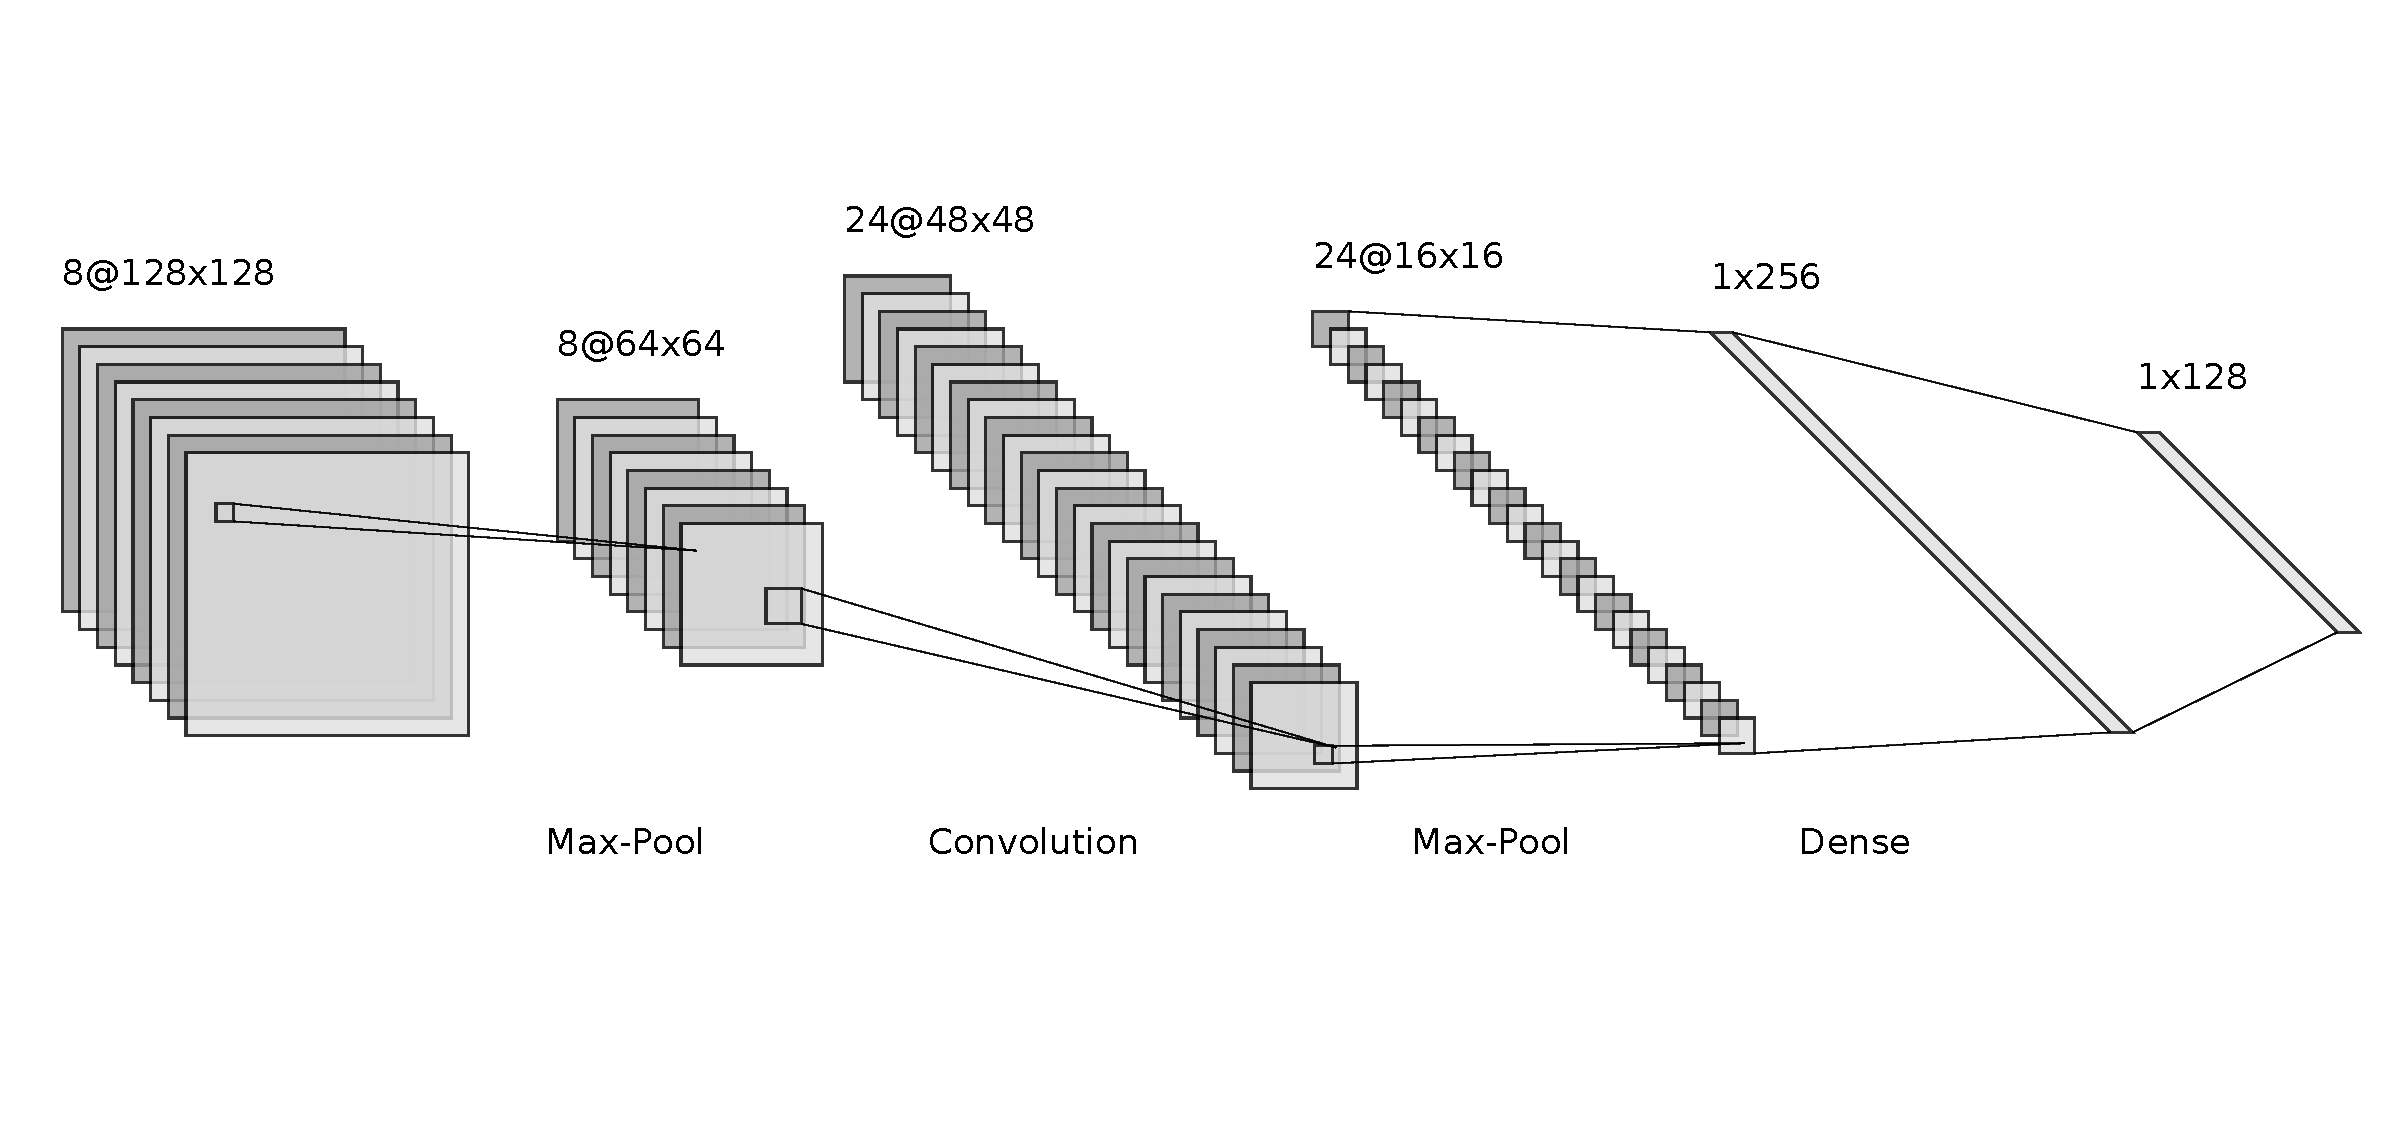
\includegraphics[width=\textwidth]{Content/fig/cnn-img.pdf}
	\caption{An example of a \ac{CNN}, abstracting some of the different layer types and connections. \label{fig:cnn}}
\end{figure}

\acp{ANN} are being increasingly used as controllers in \ac{CPS} due to their ability to learn data relationships in ways that are difficult to replicate~\cite{ANNSafety2007}. 
\acp{ANN} can deal with novel inputs to the system and are able to outperform other forms of \ac{AI} at computational efficiency, pattern recognition, function approximation and image identification~\cite{AIComp2016, AIComp2017}. 
However, it can be very difficult to ensure the safety of a system involving \acp{ANN}~\cite{ANNSafety2007, ANNSafety2018}.

\subsubsection{Training of \acfp{ANN}}
\acp{ANN} need to be trained to learn data relationships, these cannot just be made up or drawn out by hand~\cite{ann-train}.
There exist many training techniques for \acp{ANN}, all which fall under one of three categories: supervised, reinforcement and unsupervised learning.
All techniques used in this thesis fall under supervised and reinforcement learning.
Under any training method, the \ac{ANN} is trained over a training data set multiple times. 
For every time it trains over a complete data set, it is know to have trained for 1 epoch.
\acp{ANN} are often trained for thousands of epochs to converge to the best solution.

Supervised learning refers to the training when the desired output set to every input set in the training data is known.
The \ac{ANN} can be trained to converge to the correct output sets for the trained input sets.
The most well-known, and used in this thesis, supervised learning technique is back-propagation with gradient descent~\cite{grad-desc}.
This involves calculating the gradient of the error of an output set and propagating this error back through the \ac{ANN}, all the way to the inputs.
Over time, the \ac{ANN} converges to the outputs it is trained on.

However, often the desired outputs are not known.
In such systems, reinforcement learning is used to train the \ac{ANN}~\cite{reinforcement-learning}.
Reinforcement learning works by giving the \ac{ANN} a positive reward when it produces outputs that are good in its environment, and giving it negative rewards when it produces outputs that are bad. 
Thus, the \ac{ANN} can learn from good and bad decisions and learn to produce the best outputs in a given situation.

\subsubsection{\acfp{ANN} ensembles}
An \ac{ANN} ensemble is the parallel execution of multiple \acp{ANN} working in combination to produce more accurate output~\cite{Maqsood2004}.
An ensemble can contain different \acp{ANN}, with different structures, inputs, outputs and even programming languages.
The output of an \ac{ANN} ensemble represents some combination of all the \acp{ANN} in the ensemble.
The output of an \ac{ANN} ensemble is more accurate than any individual \ac{ANN} in the ensemble.
These are used to increase the prediction or classification of a system.

\subsubsection{Adversarial Perturbation in \acfp{ANN}}
A research group showed that marginal modifications to the input image of a \acf{CNN}, such as the discolouration of a few pixels, could cause the image to be misclassified~\cite{Gehr2018AI2SA, ann-pert}.
A \ac{CNN} can train to high accuracy, e.g. 99.99\%, on the training set, but simple perturbations to the \ac{CNN}'s input can lead to drastically reduced accuracy.
Figure~\ref{fig:sign-graph-acc} shows the effect of input perturbation on a \ac{ANN} trained classifier.
Misclassifications by a \ac{ANN} controller in a \ac{CPS} can have drastic consequences to the safety of the system.

\begin{figure}[h]
	\centering
	\scalebox{0.9}{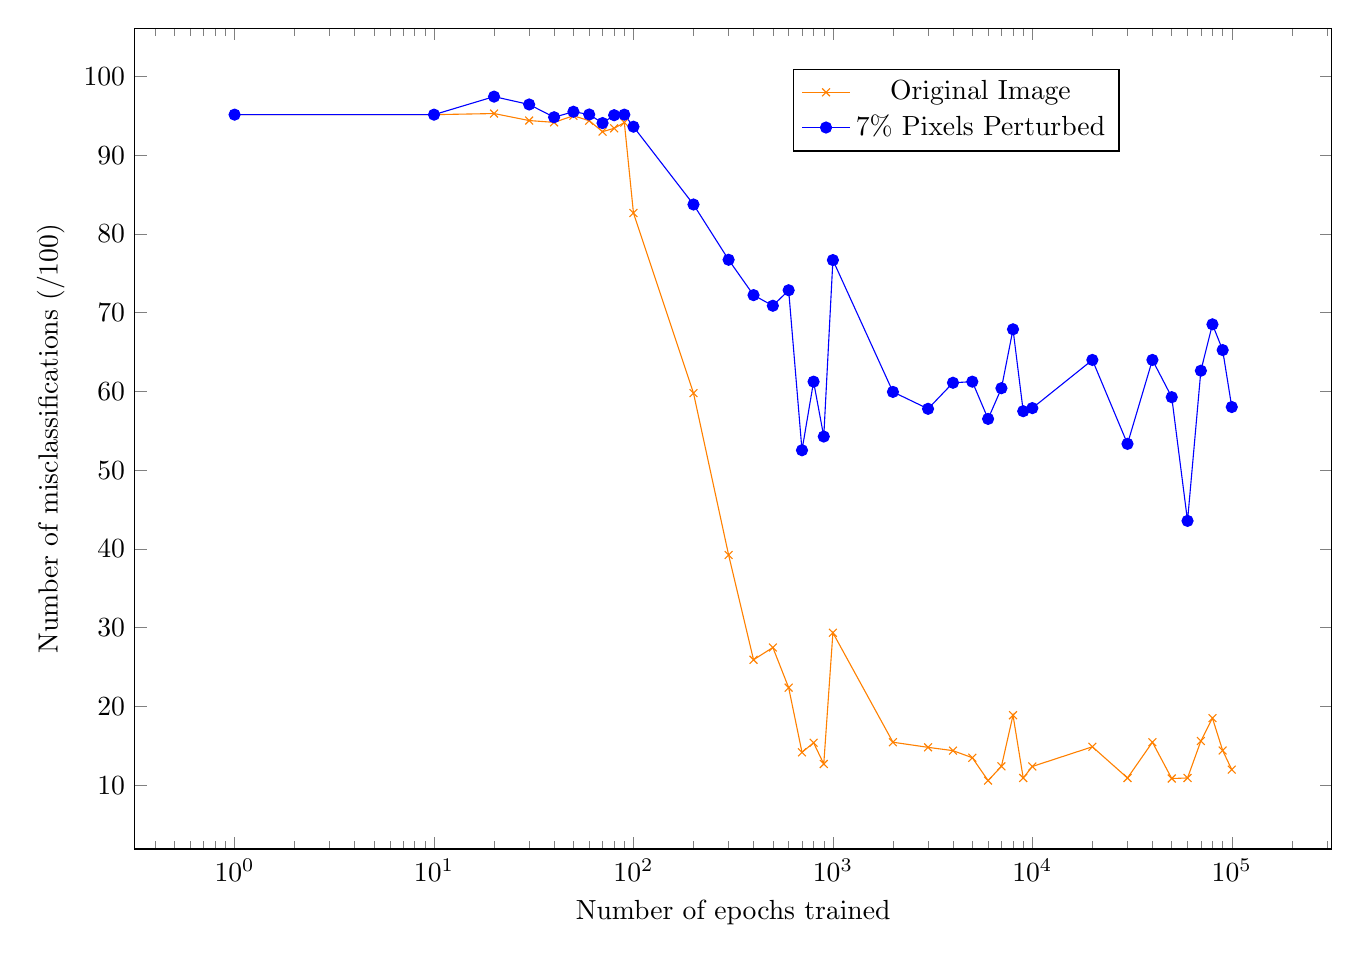
\begin{tikzpicture}
\begin{semilogxaxis}[
xlabel={Number of epochs trained},
ylabel={Number of misclassifications (/100)},
x=1.1cm,
y=1.0mm, 
legend style={at={(0.55,0.9)},anchor=west}]

\addplot[color=orange,mark=x] coordinates {
	(1, 95.159996)
	(10, 95.159996)
	(20, 95.300003)
	(30, 94.410004)
	(40, 94.180000)
	(50, 95.019997)
	(60, 94.389999)
	(70, 93.000000)
	(80, 93.419998)
	(90, 94.159996)
	(100, 82.669998)
	(200, 59.790001)
	(300, 39.240002)
	(400, 25.930000)
	(500, 27.490000)
	(600, 22.389999)
	(700, 14.180000)
	(800, 15.390000)
	(900, 12.700000)
	(1000, 29.359999)
	(2000, 15.460000)
	(3000, 14.810000)
	(4000, 14.390000)
	(5000, 13.490000)
	(6000, 10.590000)
	(7000, 12.400000)
	(8000, 18.889999)
	(9000, 10.920000)
	(10000, 12.380000)
	(20000, 14.880000)
	(30000, 10.920000)
	(40000, 15.460000)
	(50000, 10.850000)
	(60000, 10.920000)
	(70000, 15.620001)
	(80000, 18.520000)
	(90000, 14.410000)
	(100000, 11.980000)
};

\addplot[color=blue,mark=*] coordinates {
	(1, 95.159996)
	(10, 95.159996)
	(20, 97.450005)
	(30, 96.450005)
	(40, 94.830002)
	(50, 95.529999)
	(60, 95.180000)
	(70, 94.089996)
	(80, 95.089996)
	(90, 95.159996)
	(100, 93.629997)
	(200, 83.750000)
	(300, 76.729996)
	(400, 72.239998)
	(500, 70.889999)
	(600, 72.860001)
	(700, 52.540001)
	(800, 61.250000)
	(900, 54.280003)
	(1000, 76.689995)
	(2000, 59.950001)
	(3000, 57.799999)
	(4000, 61.109997)
	(5000, 61.250000)
	(6000, 56.520000)
	(7000, 60.420002)
	(8000, 67.900002)
	(9000, 57.500000)
	(10000, 57.889999)
	(20000, 64.010002)
	(30000, 53.349998)
	(40000, 64.010002)
	(50000, 59.280003)
	(60000, 43.570000)
	(70000, 62.639999)
	(80000, 68.529999)
	(90000, 65.259995)
	(100000, 58.029999)
};


\legend{Original Image, 7\% Pixels Perturbed}
\end{semilogxaxis}%
\end{tikzpicture}%}
	\caption{Line graph showing the effect of input perturbation on the prediction accuracy of a \ac{MNN} \label{fig:sign-graph-acc}}
\end{figure}

\subsubsection{\acfp{ANN} libraries used in this work}
Primarily, the our own \ac{SNN} library was used in this thesis.
This library was able to implement and train any \ac{MLP} \ac{ANN} as a time-predictable \ac{SNN}.
This library was developed in C in conjunction with the synchronous language Esterel to produce the \acp{SNN}.
However, this library was unable to handle \acp{CNN}, and we use the Darknet~\cite{darknet13} C library to implement any \acp{CNN}.
These \acp{CNN} were not time-predictable, but were able to run synchronously as \acp{SNN} using Esterel.
The Python tool-chain \acf{MNN2C} was introduced at a later stage.
This tool-chain was able to take Keras~\cite{chollet2015keras} trained \acp{ANN}, compose a \acf{MNN} from these \acp{ANN} and generate synchronous, time-predictable \acp{MNN} in C.  

\subsection{Synchronous Languages}
Synchronous languages include a variety of different languages, some notable examples being Esterel, Lustre and Signal~\cite{benveniste2003synchronous}.
When it comes to validating and implementing real-time, embedded software, synchronous languages are the most design friendly and formally sound.

Synchronous languages abide to a set of semantics, that is that they support functional concurrency, have a simple formal model and support synchrony models.
To support synchrony and concurrency, synchronous languages divide time into discrete instants according to a logical clock.
Each logical tick, the system samples the inputs, takes some action and then emits the outputs.

\subsubsection{Esterel}
Esterel is one such synchronous language, created by Gérard Berry in 1991~\cite{berry1991}. 
Esterel uses a collection of concurrently running threads synchronised to a single, global clock.
Pause statements are used to pause the thread execution, with each thread resuming from where it was paused at each clock tick.
Communication between threads is done using globally broadcast signals.
The communication between Esterel's threads is deterministic, i.e. a single signal cannot be read as both present and not present in any tick.
Esterel can, additionally, use \textit{pre()} (pre-emption) statements to check the past presence, or absence, of signals, allowing for logical delays in the execution of an action.
Due to the structure of Esterel's loops, unbounded loops are not allowed; it must be guaranteed that a loop will be paused at least once per iteration.

Figure~\ref{fig:esterel-abro} shows an \ac{ANN} run example.
This module has 2 defined input signals \textit{A} and \textit{B} and one defined output signal \textit{O}.
These signals are declared as \textit{integer} signals, meaning they have an attached integer value in addition to the presence (or absence) of the signal.
A \textit{loop} denotes an iterative thread that repeats when the \textit{end loop} statement is reached.
Each loop must include a \textit{pause}, making the loop bounded. 
The \textbf{\emph{``||''}} are used to show parallel actions, i.e. concurrency.
This means that \textit{await A} and \textit{await B} are running concurrently, where \textit{await <signal>} is synonymous with ``pause until <signal> is present''.

External functions can be called in Esterel, included from a C file.
A \textit{procedure} refers to a C function that does not return any value, while \textit{function} refers a C function that does.
The \textit{procedure runANN()(integer, integer)} takes two integers as input, and does not return any output.
The \textit{function getOutput()} takes no input, and but returns an integer as output.
The \textit{call} statement can be used to run a procedure, and just like in C the parameters are passed in brackets.
However, since \textit{A} and \textit{B} are signals, the \textbf{\emph{``?''}} is used to fetch the value at that signal, rather than the presence (or absence) of the signal.
In Esterel a \textit{function} returns some value, this value can be stored in a variable using the operator \textbf{\emph{``:=''}}, or it can be passed straight to the next function or, as with this example, be emitted by passing the parameter to the \textit{emit} statement.
The statement \textit{emit O} sets the output signal \textit{O} to be present for one tick, and sets its value according to its parameters.

When combined, the statements in this example would combine to do the following, described in English for convenience:
\begin{enumerate}
	\item Wait for A and B. 
	\item When both A and B have been present, run the function \textit{runANN} with the integer values of A and B as its parameters.
	\item Pause execution until the next tick.
	\item Emit O with the returned value of \textit{getOutput} as its integer value.
	\item Repeat from \textbf{1}.
\end{enumerate}

\begin{figure}[h]
	\begin{lstlisting}
	module ANN:
	
	procedure runANN()(integer, integer);
	function getOutput(): integer;
	
	input A: integer, B: integer;
	output O: integer;
	
	loop
	[
		[await A || await B] 
		call runANN()(?A, ?B);
		pause;
		emit O(getOutput());
	]
	end
	
	end module
	\end{lstlisting}
	\caption{An Esterel module to run a basic \ac{ANN} using C function calls.}
	\label{fig:esterel-abro}
\end{figure}

\subsection{\acf{WCET} of \acf{CPS}}
The timing analysis done in this thesis, notably \acf{WCET} analysis, is done using the Patmos controller architecture by the T-CREST project~\cite{TCREST}~\cite{patmos:ppes2011}~\cite{patmos}.
Patmos is a time-predictable processor architecture on which time-predictable software can be run and, more importantly, analysed.
Platin~\cite{compiler:platin:kps15} is a \acf{WCET} analysis tool used to calculate the \ac{WCET} of software implemented on Patmos processors.
The Platin tool is given the Patmos processor's parameters and an entry point in the C code that will be analysed.
This entry point can be any reachable C function from the \textit{main} function of the given project.
The Platin tool then compiles the C function to an intermediary file, upon which the tool uses to calculate the \ac{WCET}.
The resultant \ac{WCET} is a number of cycles on the given Patmos processor type.

However, this tool does introduce some rules to be followed for the C software to be time-predictable.
These are listed as follows:
\begin{itemize}
	\item All loops must be bounded. Every loop contained or accessed by the entry function must have a minimum and maximum number of cycles within which it will finish executing. Any \textit{for} loops are analysed by the Platin tool for the minimum and maximum, however \textit{while} loops must be given these parameters using a \textit{pragma} in the following format: \textit{pragma loopbound min <minimum> max <maximum>}. These \textit{pragmas} may also be assigned to \textit{for} loops, but this is not necessary.
	\item Dynamic memory allocation must be avoided. The use of \textit{malloc} and \textit{calloc} statements must be avoided.
	\item No C \textit{string} manipulation can be handled by Platin. This includes, but is not limited to \textit{printf} and \textit{strcpy} functions.
	\item While mathematical floating point operations can be handled by Platin, it does so very badly; i.e. a unnecessarily high \ac{WCET} is generated. As a result, floating point operations should be avoided and integer, or fixed-point, operations should be used instead.
\end{itemize}
All code generated for this thesis (except for \acp{CNN} generated using the Darknet library) adhere to this list of time-predictable rules.
Thus, all code generated for this thesis (bar Darknet \acp{CNN}) is time-predictable when implemented on a Patmos processor.

\subsection{\acf{RE} of Autonomous Systems}
While static verification has its place, more dynamic approaches to verification and safety can be used to pick up anything that the static verification and testing may have missed.
Take a standard image classification \ac{CNN} for example.
The \ac{CNN} can be trained to 99.9\% accuracy according to the test cases used to train it.
However, this means that the \ac{CNN} fails 0.1\% of the time, and that is only on the tested population, not even taking the entire population into consideration.
Having a method to verify this \ac{CNN} while it is running and pick up any inevitable failures would allow for this \ac{CNN} to be used in systems where safety is critical.

\subsubsection{\acf{RV}}
\begin{figure}[h]
	\centering
	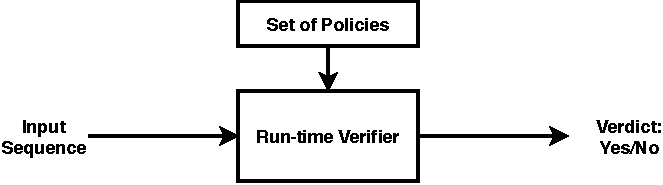
\includegraphics[width=\textwidth]{Content/fig/RV-basic.pdf}
	\caption{Basic view of a run-time verifier. \label{fig:rvbasic}}
\end{figure}

Run-time verification is an extension of run-time monitoring~\cite{runtime-verify}.
A run-time verifier monitors the I/O events of a system using a specified safety policy.
The verifier provides positive or negative feedback depending on the I/O of the system, providing a verdict for the current state of the automaton.
The run-time verifier has no knowledge of the inner workings of the system, regarding it as a black box.
This makes it ideal for autonomous systems, where the inner workings are often too complex to be verified.
Figure~\ref{fig:rvbasic} shows the basic structure of a run-time verifier.

\subsubsection{\acf{RE}}
\begin{figure}[h]
	\centering
	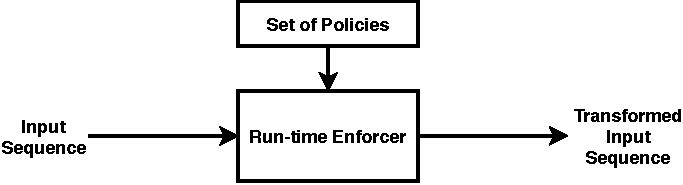
\includegraphics[width=\textwidth]{Content/fig/RE-basic.pdf}
	\caption{Basic view of a run-time enforcer. \label{fig:rebasic}}
\end{figure}

\acf{RE} is a subset of \ac{RA} that focuses on formal semantics and blocking, delaying, modifying and/or re-ordering of events in a system. 
\ac{RE} can be transformation or reactive.
Transformational \ac{RE} uses the delaying, buffering and reordering of event to enforce a safety policy, while reactive \ac{RE} uses edit functions to edit events and can be bi-directional.
This thesis focuses on reactive \ac{RE}, since \acp{ANN} are reactive in nature.
Processes that are deemed unsafe can be monitored by an enforcer at runtime to ensure that they obey desired policies and remain in a safe state at all times~\cite{theoryRE}. 
Formal runtime verification methodologies mathematically guarantee the detection of improper system behaviour \cite{RuntimeAssuranceForComplexCPS}.
For example, \ac{SA} have been proposed, which formally monitor uni-directional run-time properties only (e.g. outputs only)~\cite{enfsafepol}.
Edit automata are a type of \ac{SA} that can edit, suppress or insert events~\cite{editautomata}. 
\ac{DTA} have been proposed that can edit \textit{bi-directional} events at runtime~\cite{recps}. 
They were designed for reactive \ac{CPS} demonstrated in a pacemaker environment~\cite{recps}. 
Figure~\ref{fig:rebasic} shows the structure of a run-time enforcer.

\subsubsection{\acf{DTA} for \acf{RE}}
In order to specify the safety policies to be enforced by the run-time enforcer Pinisetty et al define \acf{DTA}~\cite{recps}.
These \ac{DTA} can be used to represent safety policies $\varphi$ which can be enforced at run-time using \textit{edit functions}~\cite{recps}.

Run-time enforcers are able to enforce binary I/O events at run-time.
I.e. the enforcers can enforce the absence or presence of an input or output signal at run-time.
A unique property of \ac{DTA} is their ability to express timed properties which can be enforced by a run-time enforcer.
A \ac{DTA} can have one or more timers, which increment at each discrete time instance.
Guards and transitions can be enforced that check the timer.
An example \ac{DTA} is given in Example~\ref{ex:dta} to introduce the syntax used in the \acp{DTA}.

\begin{figure}[h]
	\centering
	\includegraphics[]{avdta.tikz}
	\caption{\ac{DTA} example showing the syntax used to describe \acp{DTA} in this thesis\label{fig:avdta}}
\end{figure}

\begin{example}[Syntax of a \ac{DTA}]\label{ex:dta}
	The \ac{DTA} shown in Figure~\ref{fig:avdta} represents a basic safety policy.
	The policy as inputs A, B and C and output O and starts in the safe state $l_{safe}$.
	The policy's safe state transitions are described in layman's terms below: \\
	While A and B, denoted as $A~\&~B$ and not to be confused with A OR B ($A~|~B$), are present simultaneously, transition back to the safe state.\\
	However, if A and B are not detected simultaneously, transition to the unsafe state $l_{unsafe}$, suppress the output signal O ($O~:=~0$) and set the timer to 0 ($t~:=~0$).\\
	The statement $\sum\textbackslash~Z$ reads as ``anything except Z''.
	The enforcer actions are indicated by statements using the syntax $X~:=~Y$, which reads ``set X to Y''.\\
	\\
	The unsafe state has the following transitions:\\
	If the timer is less than 3 and C is not been present, transition back here while suppressing output 0.\\
	If the timer is greater than, or equal to, 3 and C is not been present, transition to the safe state.\\
	If C is detected, transition to the violation state.\\
	The absence of a signal is detected using the \textbf{overline}, e.g. ``not X'' would be $\overline{X}$.\\
	\\
	The violation state has only a single transition that returns to the violation state on anything.\\
	\\
	A brief description to the \ac{DTA} would be to say the A and B must be present together. 
	If they are not, the system is unsafe for 3 ticks, within which if C is present a violation occurs.
	After 3 ticks, the system returns to a safe state.
	While the system is in the unsafe state, the output O is suppressed by the enforcer.
\end{example}

\section{Related Work}
\subsection{\acfp{ANN} for \acf{CPS}}
In order for an \ac{ANN} to be used in any capacity within a system where safety is critical, it should undergo rigorous and thorough validation, verification, and testing procedures to ensure that they it is sufficiently safe for its target system~\cite{scann, ANNSafetyLifecycle2003}. 

While considerable research effort is starting in the direction of formal verification of \ac{AI}-based \ac{CPS}~\cite{seshia2016towards, russell2015}, the issue of timing verification has received scant attention. 
Like the challenges involving functional verification, timing verification of AI-based  \ac{CPS} poses considerable challenges due to the fact that: (1) real-time \ac{AI} systems could involve many concurrent and interacting \ac{AI} modules, which need deterministic composition for safety; (2) \ac{AI} modules are usually developed as untimed systems and the reactive nature of AI algorithms used in CPS are not carefully studied; and (3) \acf{WCET} analysis~\cite{wilhelm2008worst} of \ac{AI}-based \ac{CPS} has received scant attention.

Definitions for this safety vary, but Kurd et. al.~\cite{EstSafeCriteria2003} provide a generalisation: safe \acp{ANN} can be defined as those that:
\begin{itemize}
	\item tolerate faults and inconsistencies in their inputs,
	\item do not create hazardous outputs,
	\item behave in a predictable and repeatable manner,
	\item and are trained on clean, reliable data. 
\end{itemize}

To achieve these properties, there exist safety measures such as risk management systems that span the entire development process of the \ac{ANN}~\cite{ANNDevModel1999} and standards with which \acp{ANN} can be certified before they are used in systems where safety is critical~\cite{SCANNStandard}. 
These techniques are primarily \textit{proactive} in nature, producing \acp{ANN} that are classified as \textit{safe enough} for their role. 

However, as \acp{ANN} become larger and more full-featured, they  become harder to statically analyse.
Problematic situations can arise when an \ac{ANN} exhibits unexpected behaviour that the system is unable to safely respond to, and in \ac{CPS} these situations can be life threatening.

\subsection{Functional Verification of \acfp{ANN}}
Typical approaches for ensuring that \acp{CPS} are safe involve processes to demonstrate that an acceptable level of risk has been achieved~\cite{scann}. 
Designers of \ac{AI} software rely on several validation and verification technique, including, but not limited to, conventional testing, run-time monitoring, static analysis, model checking and theorem proving~\cite{menzies2005verification}.
Unfortunately, due to the complexity of \acfp{ANN}, techniques such as static analysis, model checking and theorem proving are less valuable in \ac{ANN} environments. 
Conventional testing is a common method to test the accuracy of \acp{ANN}, but this method is not fool-proof and its efficacy relies heavily on the creator of the test cases.
Run-time monitoring is a technique that could greatly benefit the safety of running \acp{ANN}, but there has been minimal research done in this field.

There are a variety of pre-existing methods for statically checking the correctness of autonomous (i.e. artificially intelligent) systems.
For instance, model checking on systems that use timed automata~\cite{timed-enf-autonomous}.
Okano et. al. explore the concept of model checking of autonomous systems that use timed automata~\cite{timed-enf-autonomous}.
Conventional model checking done on this automaton allowed the safety and robustness of the system to be demonstrated.
While techniques such as model checking work very well on non-\ac{ANN} \ac{AI}, \acp{ANN} are not usually able to be simplified to simple automata. 
This technique is a static technique and cannot be applied to autonomous \ac{ANN} systems, where the behaviour of the \ac{ANN} controller cannot be defined by an automaton.
For an autonomous system that includes at least one \ac{ANN} in its controller, novel techniques are required to guarantee the safety properties of the \acp{ANN}.
However, \acp{ANN} are not usually able to be simplified to simple automata.

Deep learning is a widely and extensively researched field with regards to modern machine learning that refers to the learning of data representations, rather than learning task specific algorithms~\cite{schmidhuber2015deep}.
Deep learning has applicability in a lot of current \ac{ANN} implementations, such as the autonomous vehicles used by Tesla and Uber.
Verification of \ac{ANN}, specifically, Deep Neural Networks, can be performed for certain properties (such as robustness) using \ac{SMT}~\cite{Gehr2018AI2SA,reluplex,DeepANNverify}.
This is useful, because the robustness of a deep \ac{ANN} is a critical property of its safety.
A robust \ac{ANN} is one that will provide consistently accurate outputs even when the input to the \ac{ANN} is noisy, incorrectly coloured or otherwise distorted. 
However, this approach is not flawless. 
\ac{SMT} has issues with scale: as the \acp{ANN} to analyse become larger, analysis time grows exponentially~\cite{Gehr2018AI2SA}.
Ergo, they are less efficient on larger, more complex \acp{ANN}.
In addition, they require the \acp{ANN} to fulfil some specific properties, such as specific activation functions and specific \ac{ANN} variants, i.e. \cite{Gehr2018AI2SA} only allows \acp{CNN} and \acp{MLP} with \ac{ReLU} activation functions.
This limits flexibility, as each \ac{ANN} must be designed around these restrictions, thus limiting properties of the \ac{ANN}, such as its activation function and size, could result in an \ac{ANN} that is inefficient, not robust, slow, etc.

Due to these difficulties, it can be tempting for designers to simply rely on manual testing to check for the correctness of \ac{ANN}-based systems. 
However, this is a time-consuming and error-prone process which cannot provide good guarantees, as it is very difficult to ensure that tests have acceptable coverage of all possible situations~\cite{ANN-test}.
Furthermore, as with the static analysis approaches, as the \acp{ANN} increase in size and complexity, verification and validation of these networks becomes increasingly more difficult to achieve~\cite{Gehr2018AI2SA}; test data is not unlimited, time is a resource and verification is not 100\% accurate.

Finally, no matter the chosen methodology, as \acp{ANN} increase in size and complexity, verification and validation of these networks becomes increasingly more difficult and resource intensive to achieve~\cite{Gehr2018AI2SA}.

\subsubsection{\acf{RE} of \acfp{ANN}}
% Write about exisiting autonomous RE
The idea of \ac{RE} of autonomous systems has received some research attention. 
De Niz et. al. propose a type of \ac{RE} they term temporal enforcement, which ensures that the system controller meets timing deadlines where outputs are concerned~\cite{safe-enforce-auto}. 
While this shares similarities with the work in this paper, their work does not expand to cover \acp{ANN}, and does not propose the use of \ac{RE} for anything other than meeting timing deadlines.
Aniculaesei et. al. propose static formal verification and runtime monitoring of autonomous, robotic systems to prevent physical collisions during system execution~\cite{runtime-monitor}.
While this looks at the enforcement of system outputs, the inputs are not monitored and the timing deadlines of the system are not investigated. 
Additionally, the case study involves a robot controlled by an automaton, not a highly complex \ac{AI} such as an \ac{ANN}.
